\chapter{矩阵定理}

\section{向量性质}

\subsection{基本性质}

\paragraph*{内积与夹角}在二维平面上,内积的含义是平行四边形的有向面积.

$$\cos\theta=\frac{\bx\cdot\by}{|\bx||\by|}$$

$\theta$为夹角.夹角与欧几里得距离有关联.考虑端点在单位圆上的两个向量$\bx_1,\bx_2$.则两个端点的欧几里得距离为:

$$2\sin\frac{\theta}{2}=2\sqrt{1-\cos^2\frac{\theta}{2}}$$

参考下图:

\begin{center}
	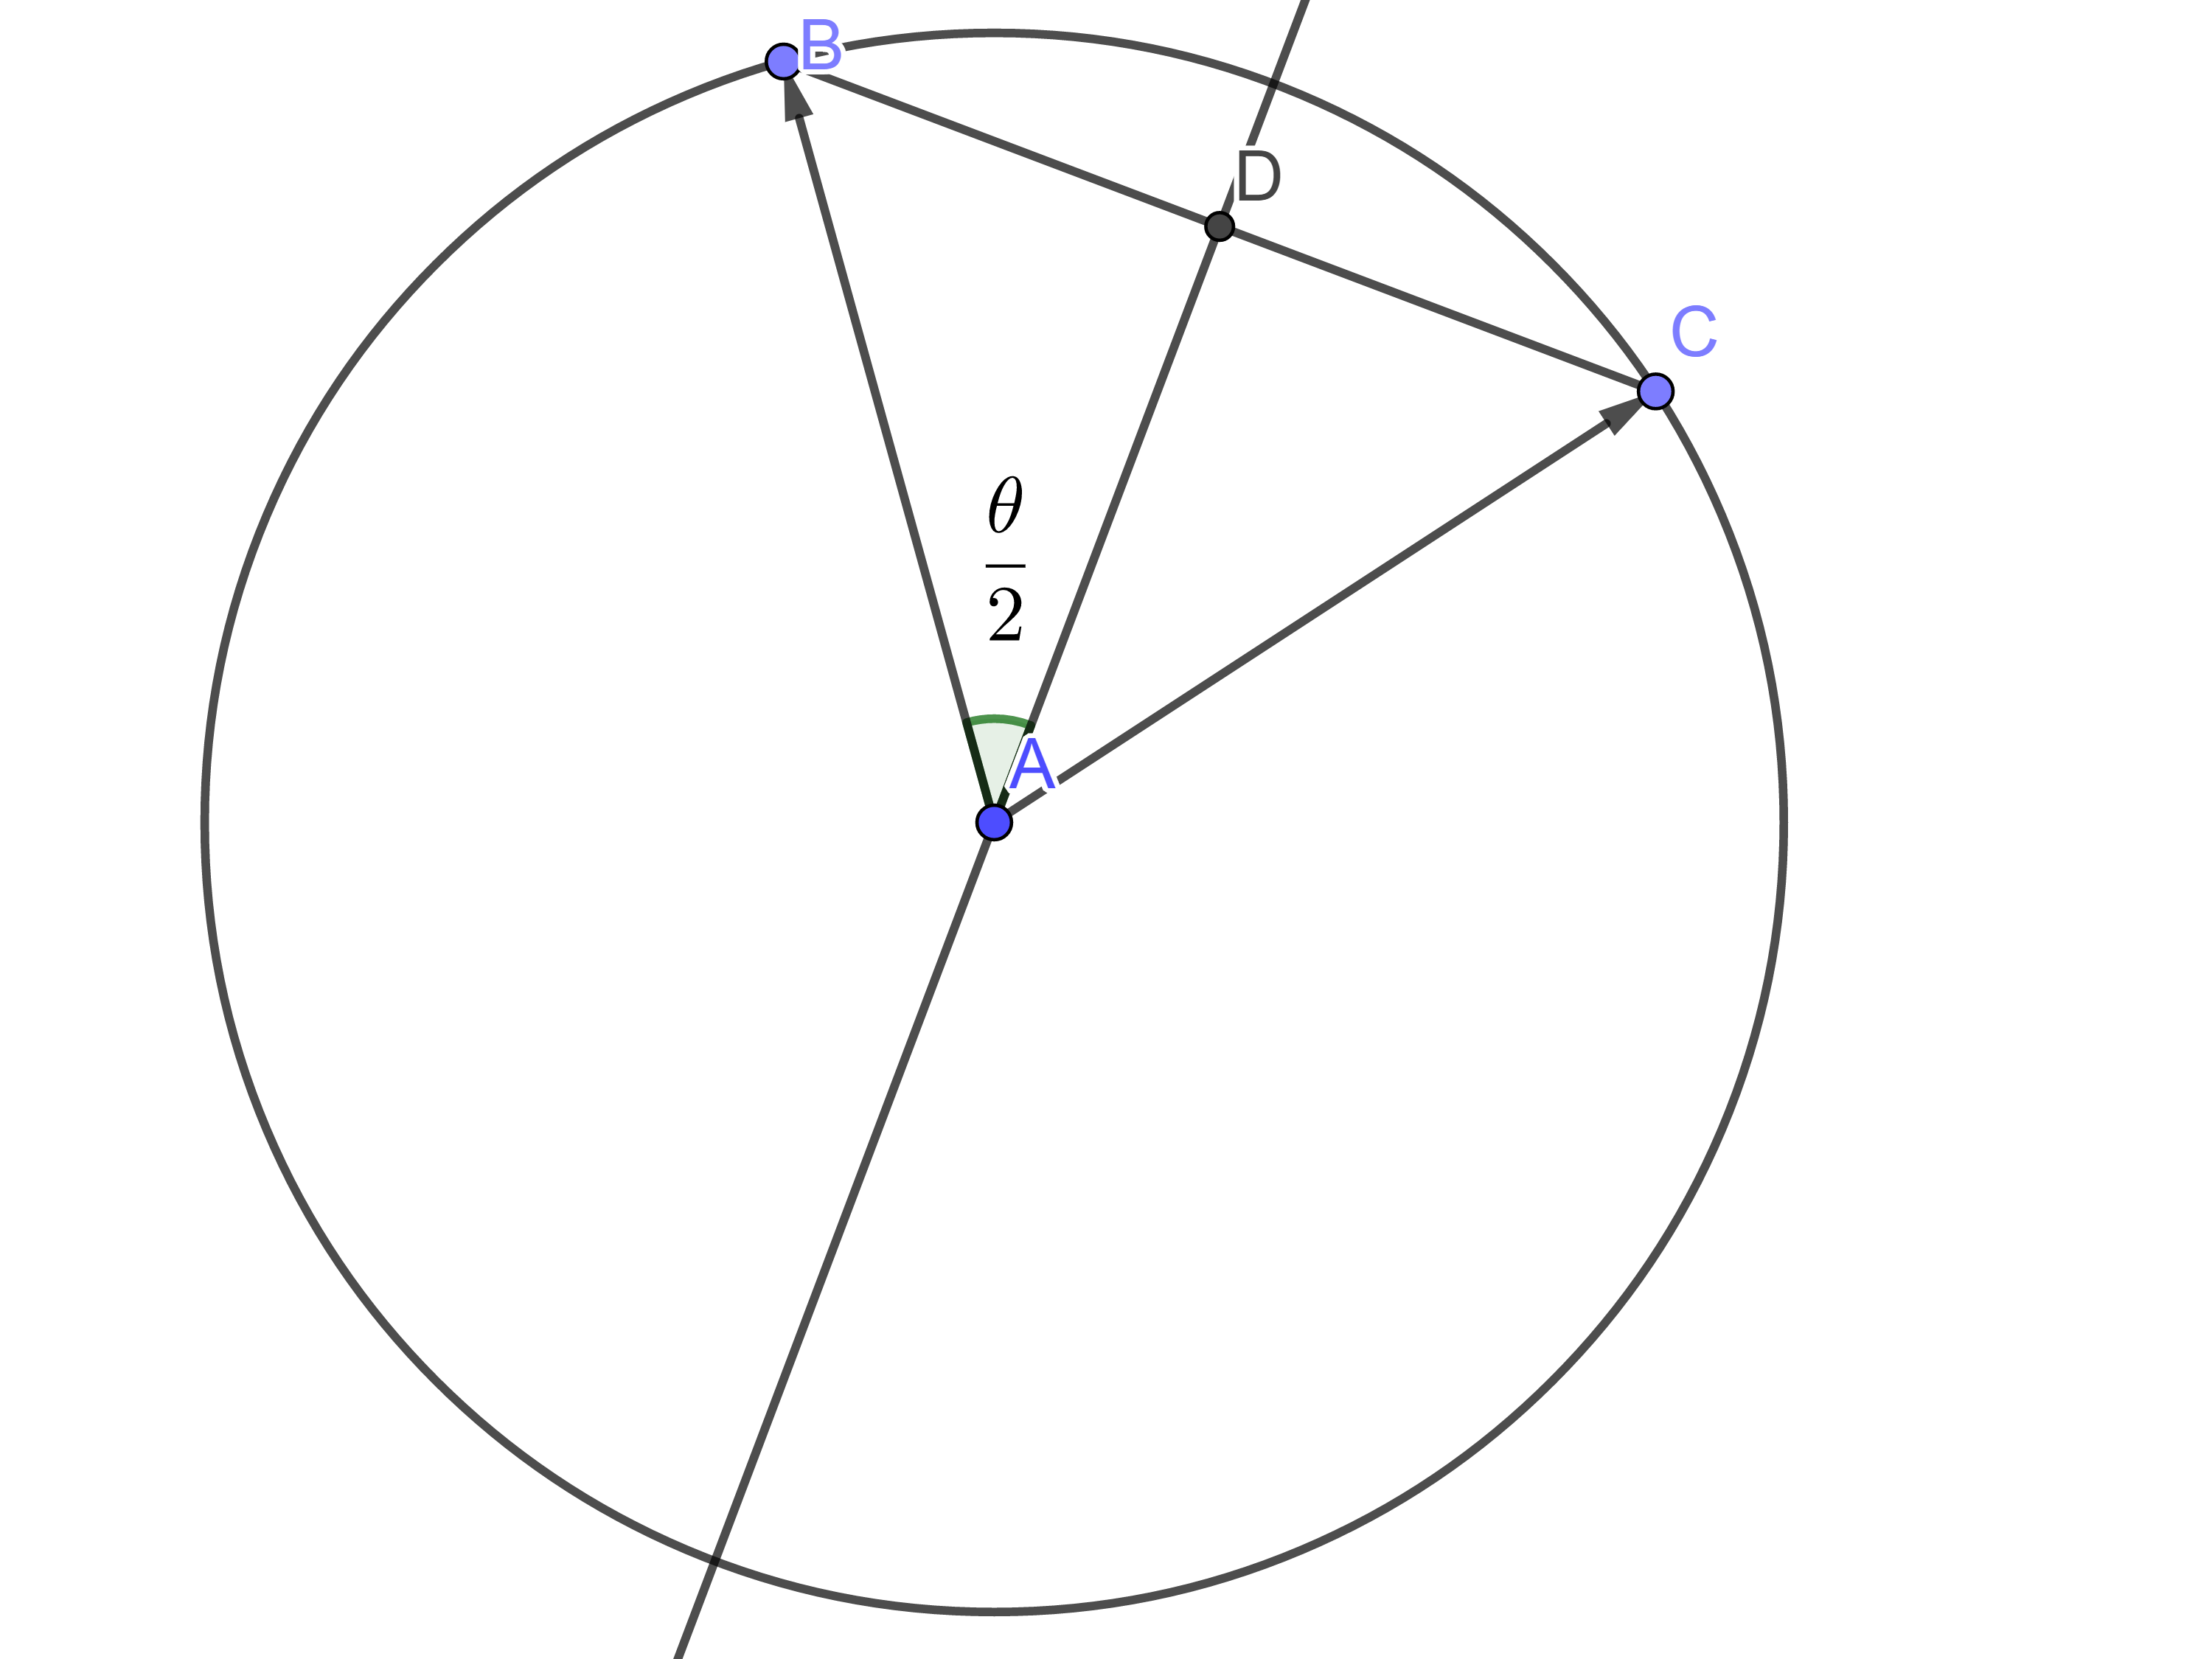
\includegraphics[width=6cm]{figure/cosDistance.png}
\end{center}

\paragraph*{垂直(orthogonal)}垂直关系可以用内积描述:

$$\bx\cdot\by=0$$

如果另外有$|\bx|=|\by|=1$,则称为orthonomal.
\section{矩阵性质}

\subsection{逆矩阵}
$$A^{-1}=\frac{1}{|A|}A^{\star}$$
其中$A^{\star}=M^T$为伴随矩阵,其值为
$$M_{ij}=(-1)^{i+j}|A_{-i,-j}|$$
$M_{-i,-j}$为去掉矩阵的$i$行$j$列后剩下的矩阵。

$n$阶可逆矩阵构成一般线性群$\GL_n$。对于2阶矩阵有简单的表达式:
$$\begin{bmatrix}
a&b\\c&d
\end{bmatrix}=\frac{1}{ad-bc}\begin{bmatrix}
d&-b\\-c&a
\end{bmatrix}$$
注意
$$M=\begin{bmatrix}
	d&-c\\-b &a
\end{bmatrix}$$
转置一下就是上面的表达式。求二阶线性方程组的时候可以用。

手动计算矩阵逆时可以使用消元法,首先构造矩阵$(A,I)$,通过行变换变成$(I,A')$,则$A'=A^{-1}$。具体操作时,首先把$A$的下半部分变成全0,依次把第1列的$2,\cdots,n$行元素变成0,然后把第2列的$3,\cdots,n$个元素变成0,$\cdots$再变换上半部分为全0。
\subsection{特征向量与特征值}
\subsubsection{定义}
特征值集合在算子理论中也叫做谱,用$\sigma(A)$表示,通常将特征值从大到小排列,那么$\lambda_1=\sigma_1(A)$就表示最大的特征值,$\lambda_n=\sigma_n(A)$为最小特征值。常用的特征值只对\textbf{方阵}才有定义。

\begin{empheq}{align*}
	A\bx&=\lambda\bx\\
	\sum \lambda_i &=\trace A\\
	\prod \lambda_i &=\det A
\end{empheq}

特征值的最大模就是谱半径:

\begin{definition}[谱半径]\label{matrix-spec-radius}
\begin{equation}
\rho(A)=\max_i |\lambda_i(A)|
\end{equation}
\end{definition}
要注意区别谱半径与谱范数,谱半径不是矩阵范数,但它非常重要。

谱半径有一个重要性质:
$$\rho(A)\leq\|A\|$$
即它小于任意一种范数。同时还有Gelfand定理:
\begin{equation}
\rho(A)=\lim_{k\rightarrow \infty} \|A^k\|^{1/k}
\end{equation}

\subsubsection{特征值和特征向量性质}
\begin{enumerate}
\item  常见矩阵函数的特征值:
\begin{longtable}{|c|c|c|c|c|}
\hline
矩阵& $A$& $A^T$& $A^{-1}$& $A^k$\\
\hline
特征值& $\lambda$ & $\lambda$ & $\inv{\lambda}$ & $\lambda^k$\\
\hline  
\end{longtable}
如果$A$有SVD分解$A=U\Lambda V$,即$A$有奇异值$\sigma_i$,则$AA^T$的特征值为$\lambda_i=\sigma_i^2$。
\item 如果已知特征值和特征向量,则从$A$中去掉一行,右边的特征向量中去掉对应的行,等式依然成立.
\item 假设$A\in\mathbb{R}^{d\times n},B\in\mathbb{R}^{n\times d},d\leq n$,即$A$为横矩阵,则$AB$为小方阵,有$\sigma(BA)=(\sigma(AB),\bm{0})$,特别地,假如$d=n$,那么$\sigma(AB)=\sigma(BA)$。

对于三个矩阵,在矩阵乘法成立的情况下,有$\sigma(ABC)=\sigma(BCA)=\sigma(CAB)$。在二次型定理\ref{quadratic-form-ratio}的证明中就会用到:
$$\sigma(B^{-1}A)=\sigma(R^{-1}(R^{-T})A)=\sigma(R^{-T}AR^{-1})$$
\item 如果$A$是Hermitian矩阵,则
\begin{empheq}{align}
\lambda_1&=\max_{\|\bx\|=1}\bx^TA\bx\\
\lambda_n&=\min_{\|\bx\|=1} \bx^TA\bx\\
\end{empheq}

更一般地有:
\begin{empheq}{align}
\sum_{i=1}^k \lambda_k&=\underset{(\bx_1,\cdots,\bx_k)}{\max}\sum_{i=1}^{k}\bx_i^TA\bx_i \mtag{Ky Fan's Maximum Principle}\\
\sum_{i=n-k+1}^n \lambda_k&=\underset{(\bx_1,\cdots,\bx_k)}{\min}\sum_{i=1}^{k}\bx_i^TA\bx_i \mtag{Ky Fan's Maximum Principle}\\
\end{empheq}
要求$(\bx_1,\cdots,\bx_k)$相互orthonormal。
\end{enumerate}

\subsubsection{迭代算法}
\paragraph*{计算最大的特征值与特征向量}
\begin{empheq}{align}
\bx_{n+1}&=\alpha(A\bx-\bx^T\bx\bx)+\bx
\end{empheq}
收敛时$\bx$就是特征向量,对应特征值$\bx^T\bx$。

\paragraph*{计算最小的特征值与特征向量}
\begin{empheq}{align}
\bx_{n+1}&=\alpha((kI-A)\bx-\bx^T\bx\bx)+\bx
\end{empheq}

\subsection{奇异值}
SVD分解中$\Lambda$矩阵的对角元素就是奇异值。

\subsubsection{与特征值的联系}
\begin{enumerate}
\item 
$$\sigma_i^2(A)=\lambda_i(A^*A)=\lambda(AA^*)$$
\item 对于$n$阶矩阵:
$$\lambda_i(A+A^*)\leq 2\sigma_i(A)$$

假如$A$是对称的,则有
$$\lambda_i(A)\leq\sigma_i(A)$$
\item 正定矩阵的特征值与奇异值相同。
\end{enumerate}
\subsubsection{$A+B$的奇异值}
\begin{enumerate}
\item $A+B,A,B\in\mathbb{C}^{m,n}$的奇异值:
$$\sigma_{i+j-1}(A+B)\leq \sigma_i(A)+\sigma_j(B),i+j-1\leq \min\{m,n\}$$

特殊情况:
\begin{enumerate}
\item 假如取$m=n$,分别令$i=1,j=n$和$i=n,j=1$,有:
\begin{empheq}{align*}
\sigma_n(A+B)\leq \sigma_1(A)+\sigma_n(B)\\
\sigma_n(A+B)\leq \sigma_n(A)+\sigma_1(B)\\
\end{empheq}
\end{enumerate}
\end{enumerate}

\subsection{矩阵范数}
矩阵范数对任何矩阵均存在,且任何矩阵范数都是等价的。

\subsubsection{范数的类型}
\paragraph*{Unitarily invariant norm}比较常用的类型。
\begin{definition}[Unitarily invariant norm]
一个范数如果满足
$$\forall A,\|UAV\|=\|A\|$$
其中$U,V$为任意酉矩阵。则称之为Unitarily invariant norm。

Frobenius范数都属于此类。
\end{definition}

\subsubsection{诱导范数}
参考算子范数\ref{op-norm},它依赖于向量的范数。如果向量取$p$范数,则有相应的$\|A\|_p$。特殊情形:
\begin{description}
\item[$p=1$] 列范数,先把所有元素取绝对值,再对每列求和,然后取最大的。
\item[$p=2$] 谱范数,参见\ref{matrix-spec-norm}。
\item[$p=\infty$] 行范数。与列范数相对应。
\end{description}
\subsubsection{谱范数}
\begin{definition}[谱范数]\label{matrix-spec-norm}
$$\|A\|_2=\sigma_{\max}(A^TA)$$
即最大奇异值。注意$A$不必是方阵。
\end{definition}
\begin{property}
\begin{enumerate}
\item 根据奇异值分解可得:
$$\|A^{-1}\|=\inv{\min \sigma(A)}$$
\end{enumerate}
\end{property}

\subsubsection{Frobenius范数}
\begin{definition}[Frobenius范数]
对于一个长方阵$X\in\mathbb{R}^{n\times d}$,有Frobenius范数:
\begin{empheq}{equation}
\|A\|_F=\sqrt{\trace(A^TA)}=\sqrt{\trace(AA^T)}=\sqrt{\sum |A_{ij}|^2}
\end{empheq}
最后一个等号说把所有元素排列一个向量,然后取向量的$L_2$范数。

显然从定义可以看出
$$\|A\|_2\leq \|A\|_F$$
\end{definition}

\subsection{特殊矩阵}
\subsubsection{常见复矩阵及对应的实矩阵}
记$A^H$为伴随矩阵,是复矩阵的共轭转置、实矩阵的转置($A^T$),有时也用$A^*$表示.

\begin{longtable}{c c}
	\toprule
	名称& 定义 \\
	\midrule
	Hermitian(对称矩阵) &$A=A^H$ \\
	斜伴矩阵(反对称矩阵)&$A=-A^H$\\
	正规矩阵& $AA^H=A^H A$\\
	酉矩阵(正交矩阵)& $AA^H=A^H A=I$\\
	\bottomrule
\end{longtable}

\paragraph*{Hermitian}具有非常重要的性质:
\begin{enumerate}
\item 如果元素全为实数,则为实对称阵。满足性质:
\begin{enumerate}
\item 实对称矩阵必然可以对角化。
\item 不同特征值对应的特征向量正交。
\item 特征值必为实数。
\end{enumerate}
\end{enumerate}
\subsubsection{正矩阵与非负矩阵族}
\paragraph*{非负矩阵}元素非负的矩阵,不要与负定矩阵混淆。

\begin{definition}[非负矩阵]
对于矩阵$A$,如果$A_{ij}\geq 0$,称$A$为非负矩阵,记为$A\geq 0$。我们用$|A|$表示按元素取绝对值。

非负矩阵具有以下性质:
\begin{enumerate}
\item 如果$B\geq A\geq 0,D\geq C\geq 0$,则$BD\geq Ac\geq 0$
\item 如果$B\geq A\geq 0$,则$B^k\geq A^k\geq 0,k=1,2,\cdots$。
\item 如果$|A|\geq B$,则$\rho(A)\leq\rho(|A|)\leq \rho(B)$。
\end{enumerate}
\end{definition}


\paragraph*{Z矩阵与M矩阵}
\begin{definition}[Z矩阵与M矩阵]\label{z-m-matrix}
记方阵$A=[A_{ij}]\in\mathbb{R}^{n\times n}$,如果$A_{ij}\leq 0,i\neq j$(非对角元素小于等于0),则称$A$为$Z$矩阵,任何一个$Z$矩阵$A$可以表示成$A=sI-B$,且$s>0,B\geq 0$。

如果$s\geq \rho(A)$,称$A$为$M$矩阵。若$s>\rho(B)$,称之为非奇异$M$矩阵,$s=\rho(B)$时,称为奇异的$M$矩阵。

$\rho(A)$为谱半径\ref{matrix-spec-radius}。
\end{definition}

\begin{theorem}[Z矩阵的性质]
若$A$为$Z$矩阵,则下列命题等价:
\begin{enumerate}
\item $A$是非奇异的$M$矩阵。
\item $A$非奇异且$A^{-1}\geq 0$。
\item 存在$\bx>0$使得$A\bx>0$。
\item 任意$\lambda\in\lambda(A)$,有$\Re(\lambda)>0$。即特征值的实部为正。
\item $A$的所有实特征值都是正数。
\end{enumerate}
\end{theorem}
\subsubsection{正定矩阵与二次型}
\paragraph*{定义}
\begin{definition}[正定矩阵]\label{pos-definite-matrix}
对称矩阵$A$如果满足
$$\forall \bx\in\mathbb{R}^n,\bx^TA\bx> 0$$
称$A$为正定矩阵,如果取$\geq$,就是半正定矩阵,如果取$<$,就是负定矩阵。,单位阵是半正定矩阵。

正定矩阵也可以表示为$A\succ 0$,半正定矩阵就是$A\succeq 0$。有的地方也用$A\geq 0$来表示半正定矩阵,但这容易与非负矩阵混淆。

\end{definition}
\paragraph*{性质}正定矩阵满足以下性质:
\begin{enumerate}
\item 行列式为正。这是由于特征值非负,特征值的乘积就是行列式。
\item 对角线元素之和为正。因为特征值之和为对角线元素之和。
\item 特征值全部为正。
\item 正定矩阵之和仍然正定,Hadmond积也正定(Schur乘积定理),但矩阵乘积\textbf{可能不正定}:
\begin{empheq}{equation}
A\succ 0,B\succ 0\implies A+B\succ 0, A\odot B\succ 0
\end{empheq}
\item 正定矩阵的逆正定:$A\succ 0\implies A^{-1}\succ 0$。再加上上一条,可以导出:如果$A\succ B\succ 0$,则$A+B\succ B$,然后有$(A+B)^{-1}\succ B^{-1}$。
\item 对于两个正定矩阵$A,B$,有和矩阵的特征值:
$$\lambda_k(A)+\lambda_n(B)\leq \lambda_k(A+B)\leq \lambda_k(A)+\lambda_1(B)$$
$\lambda_1$为最大的特征值,$\lambda_n$为最小特征值。特殊情况:
\begin{empheq}{align*}
\lambda_n(A)+\lambda_n(B)&\leq \lambda_n(A+B)\leq\lambda_n(A)+\lambda_1(B)
\end{empheq}

有矩阵乘法的特征值:
\begin{empheq}{align*}
\lambda_1(AB)&\leq \lambda_1(A)\lambda_1(B)\\
\lambda_n(A)\lambda_n(B)&\leq \lambda_n(AB)
\end{empheq}
\end{enumerate}


涉及正定或者半正定矩阵的其它一些定理:
\begin{enumerate}
\item 如果$A$非负定,则
$$(\bx^TA\by)^2\leq(\bx^TA\bx)(\by^TA\by)$$
\item 如果$A$正定,则
$$(\bx^T\by)^2\leq (\bx^TA\bx)(\by^TA^{-1}\by)$$
\item 如果$A$非负定,则
$$|A_{ij}|\leq \max \{A_{ii}\}$$
也就是说非负定矩阵中绝对值最大的元素位于对角线上。
\item 非负定矩阵$A,B$满足:
\begin{empheq}{align}
0\leq \trace(AB)&\leq \trace(A)\trace(B)\\
\det(A+B)&\geq \det(A)+\det(B) 
\end{empheq}
对于第2式,如果$n\geq 2$且$A,B$正定,则只取$>$。
\item 如果$A,B,C,D,U,V$都是同样大小的方阵,且$U,V$正定,则
$$\det(AUA^T+BVB^T)\det(CUC^T+DVD^T)\geq \det(AUC6T+BVD^T)^2$$
\item 如果$A$非负定,则
$$\det(I+A)\geq 1+\det(A)$$
如果$n\geq 2$且$A$正定,则只取$>$。
\end{enumerate}

\paragraph*{判定}判断一个对称矩阵是否正定:
\begin{enumerate}
\item 顺序主子式为正。就是取前$k$行$k$列,计算行列式。左上角元素就是第1个顺序主子式,所以要求这个元素为正。

如果奇数阶主子式为负(第一个元素为负),偶数阶为负,就是负定矩阵。

此外需要注意,假如顺序主子式全部非负,不一定半正定。
\end{enumerate}

\paragraph*{二次型}
\begin{enumerate}
\item 对于任意对称方阵$A$,
\begin{empheq}{align*}
\max_{|bx|=1}\bx^TA\bx=\lambda_{\max},&\quad \min_{|bx|=1}\bx^TA\bx=\lambda_{\min}\\
\max_{bx}\frac{\bx^TA\bx}{\bx^T\bx}=\lambda_{\max},&\quad \min_{bx}\frac{\bx^TA\bx}{\bx^T\bx}=\lambda_{\min}\\
\end{empheq}
\item\label{quadratic-form-ratio} $A,B$为任意$n$阶方阵, $B$正定,则有
$$\max_{\bx\neq\bm{0}} \frac{\bx^TA\bx}{\bx^TB\bx}=\lambda_{\max}(B^{-1}A)$$

\end{enumerate}
\subsubsection{投影矩阵}
给定一个行满秩矩阵$A\in \mathbb{R}^{m\times n},m\leq n$,现在有一个向量$\bx\in\mathbb{R}^n$,希望将它投影到$A$的零空间。

首先可以这样考虑,求一个向量$\bx'$,它满足零空间的定义,同时尽量接近$\bx$,可以形式化为一个最小二乘问题:
\begin{empheq}{equation}
\begin{aligned}
	\min_{\bx'\in\mathbb{R}^n} & \inv{2}(\bx'-\bx)^T(\bx'-\bx)\\
	\text{s.t. }& A\bx'=\bm{0}
\end{aligned}
\end{empheq}
目标函数是距离。用乘子法:
\begin{empheq}{align*}
L(\bx',\bm{v})&=\inv{2}(\bx'-bx)^T(\bx'-\bx)+\bm{v}^TA\bx',\bm{v}\in\mathbb{R}^m\\
\pdv{L}{\bx'}&=\bx'-\bx+A^T\bm{v}=0\\
A\bx'&=\bm{0}
\end{empheq}
第二个式子左乘$A$,就可以得到
$$\bm{v}=(AA^T)^{-1}A\bx$$

同时由第二个式子有$\bx'=\bx-A^T\bm{v}$,于是
$$\bx'=P\bx=(I-A^T(AA^T)^{-1}A)\bx$$
$P=I-A^T(AA^T)^{-1}A,P\in\mathbb{R}^{n\times n}$称为投影矩阵。

也可以从另一个角度考虑,希望求解$\bx$在$A$的零空间下的坐标。

\subsubsection{Stiefel流形}
Stiefel流形是正交矩阵的扩展,它的定义为
\begin{empheq}{equation}
\mathcal{S}_{n,d}\{A\in\mathbb{C}^{n\times d}:A^HA=I\}
\end{empheq}
注意它不必是方阵。

\paragraph*{性质}Stiefel流形具有以下性质:
\begin{enumerate}
\item $\dim(\mathcal{S}_{n,d})=nd-\inv{2}d(d+1)$
\end{enumerate}

\subsection{矩阵分解}
\subsubsection{概览}
\begin{longtable}{m{0.15\textwidth} m{0.15\textwidth} m{0.3\textwidth} m{0.4\textwidth}}
	\toprule
	\hfil \textbf{范围}&\hfil \textbf{名称} & \hfil \textbf{形式}  & \hfil \textbf{说明}\\
	\midrule
任意矩阵 &	SVD分解 &$A_{m\times n}=U_{m\times m}\Lambda_{m\times n}V_{n\times n}$&$U,V$酉矩阵,$\Lambda$实对角阵,其中的元素为奇异值。\\
任意方阵&Jordan标准型 &$A=PJP^{-1}$ &$J=\diag(J_1,J_2,\cdots)$,其中$J_k$的对角线上全为$\lambda_k$,且对角线右边的一个元素全为1。形如:
$$J_k=\begin{bmatrix}
\lambda_k & 1 & &\\
& \lambda_k& 1 & & \\
& & \cdots& &\\
& & & &\lambda_k
\end{bmatrix}$$ \\
\hline
	任意方阵 &QR分解&$A=QR$ & $Q$正交,$R$上三角\\
    \hline
某些方阵& 对角化 &$A=Q\Lambda Q^{-1}$&$\Lambda$为对角矩阵,对角线上元素为特征值。$Q$的列为特征向量,显然如果要$Q$可逆,则特征空间的维数必然等于$n$。

强调实对称矩阵必然可以对角化。\\
\hline
    任意方阵& Schur分解 &$A=QUQ^{H}$ & $Q$酉矩阵,因此 $Q^{-1}=Q^H$,$U$半上三角阵,对角线上为$A$的特征值.\\
    \hline
	半正定矩阵& Cholesky分解& $A=LL^H $& $L$下三角.\\
	\bottomrule
\end{longtable}

\subsubsection{SVD分解}
\paragraph*{低秩逼近}SVD分解的一个重要应用是用低秩矩阵逼近一个目标矩阵,其最优逼近为
$$A_k=\sum_{i=1}^k\lambda_i \bm{u}_i\bm{v}_i^T$$
$\bm{u}_i$是$U$的列,$\bm{v}_i$是$V$的列。
\section{线性方程组的解}
\subsection{齐次方程组}
一个齐次线性方程组形如:
$$A\bx=\bm{0}$$
$A\in \mathbb{R}^{m\times n}$,$m$是方程个数,$n$是变量个数。
\begin{enumerate}
\item 显然,这个方程组至少有1个解:$\bm{0}$解,即$\bx=\bm{0}$。
\item 假如$\rank(A)=n$,即列满秩,则只有$\bm{0}$解。列满秩时,列之间是独立的,所以不可能找到一个线性组合使和为0.
\item 假如$\rank(A)<n$,则有无穷多个解。此时解空间又称为$\nullspace$(或者叫kernel),满足条件:
$$\dim(\nullspace(A))+\rank(A)=n$$
零空间的基相当于方程组基础解系,$\dim(\nullspace(A))$就是基变量的个数。
\end{enumerate}
\subsection{非齐次方程组}
对于一个非齐次方程组
$$A\bx=\bm{b}$$
其增广矩阵为$(A,\bm{b})$。解的存在性由以下判别方法给出:
\begin{enumerate}
\item $\rank(A)< \rank(A,\bm{b})$,则无解。
\item $\rank(A)= \rank(A,\bm{b})<n$,有多个解。
\item $\rank(A)= \rank(A,\bm{b})=n$,唯一解。
\end{enumerate}